\documentclass[UTF8]{ctexart}
\usepackage[top=1.2in,bottom=1.2in,left=1.25in,right=1in]{geometry}
\usepackage{hyperref}
\usepackage{graphicx}

\title{SSH 目录不可创建文件问题修复}
\author{}
\date{\today}

\begin{document}

\maketitle

\newpage

\section{问题发现}
最开始发现问题是使用 apt 更新软件
\begin{figure}[ht] 
	\centering
	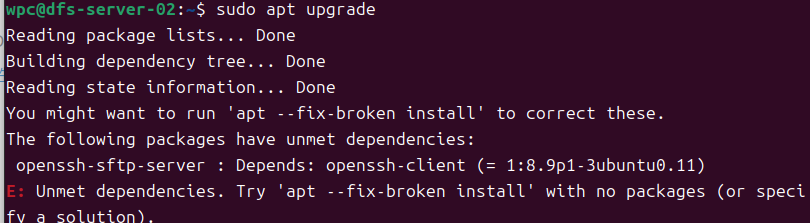
\includegraphics[scale=0.5]{1.png}
	\label{}
\end{figure}

尝试运行 \verb|apt --fix-broken install| 修复问题
\begin{figure}[ht] 
	\centering
	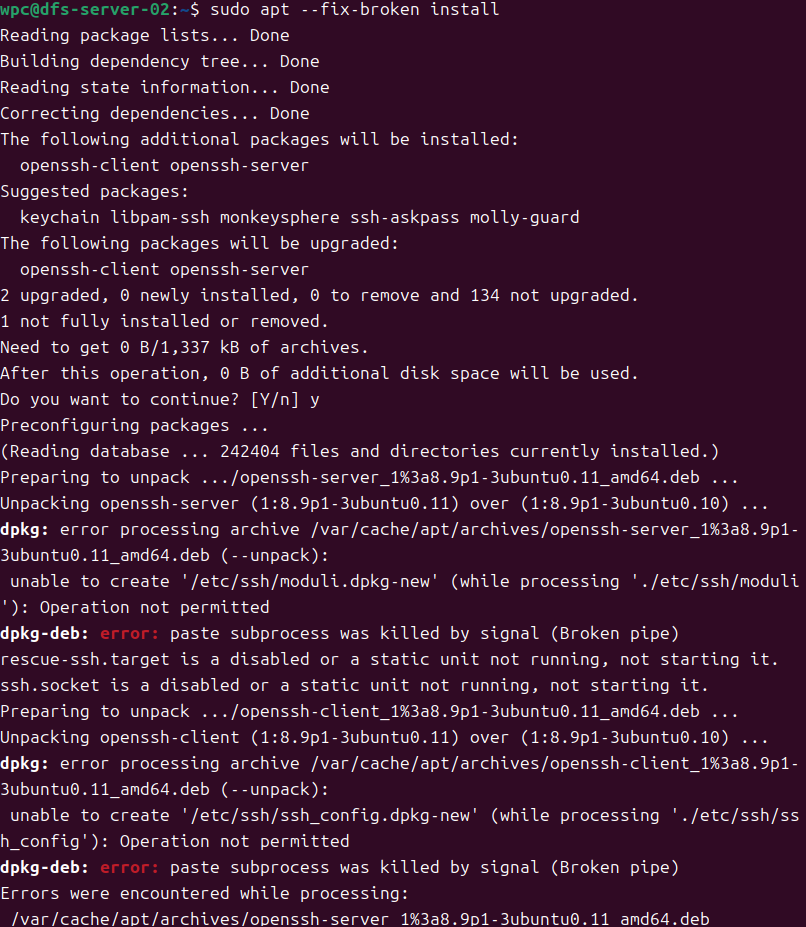
\includegraphics[scale=0.5]{2.png}
	\label{}
\end{figure}

\section{着手修复}
观察控制台输出，可知是 openssh-server 和 openssh-client 两个软件包的问题，尝试重装这两个软件包
\begin{enumerate}
    \item 卸载包：
    \begin{verbatim}
    sudo apt remove openssh-server openssh-client --purge 
    sudo apt autoremove 
    sudo apt autoclean
    \end{verbatim}
    
    \item 仍有 error，强制删除：
    \begin{verbatim}
    sudo dpkg -P --force-all openssh-server openssh-client
    \end{verbatim}

    \item 尝试修复：
    \begin{verbatim}
    sudo apt-get install -f
    \end{verbatim}
\end{enumerate}
经过上述步骤，问题仍没解决，不过输出的 error 少了许多，openssh-server 的问题已经解决，但 openssh-client 仍有问题
\begin{figure}[ht] 
	\centering
	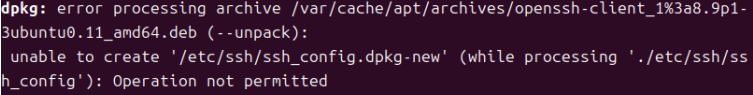
\includegraphics[scale=0.5]{3.png}
	\label{}
\end{figure}

\section{问题分析与修复}
从控制台输出看出问题出在无法创建文件上，尝试手动创建文件
\begin{verbatim}
    cd /etc/ssh
    touch ssh_config.dpkg-new
\end{verbatim}
出现 error，touch: setting times of `xxx': No such file or directory

使用 ls 查看 /etc/ssh 目录权限，并未发现问题，
\begin{figure}[ht] 
	\centering
	
\includegraphics[scale=0.5]{4.png}
	\label{}
\end{figure}

估计是设置了隐藏属性，使用 lsattr 查看目录属性，发现目录被锁定
\begin{figure}[ht] 
	\centering
	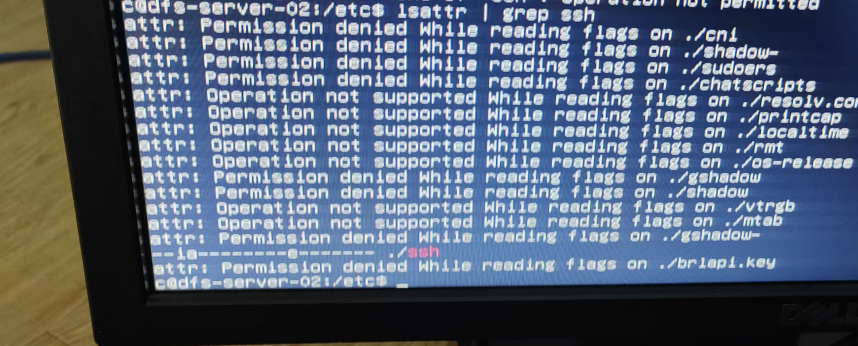
\includegraphics[scale=0.5]{5.png}
	\label{}
\end{figure}
使用 chattr -ia ./ssh 修复问题，到此问题解决

\end{document}
